\icode{E-MD-CA-L2-261114-008}
如图所示，在水平地面上固定一倾角为\qty{37}{\degree}足够长的斜面，今有一木块以初速度\qty{8}{m/s}冲上斜面，木块与斜面的动摩擦因数为 $0.25$，（最大静摩擦力近似等于滑动摩擦力，\(\sin\)\qty{37}{\degree}= 0.6，\(\cos\)\qty{37}{\degree}= 0.8，（\(g =\) \,\qty{10}{m/s^2}）则：
\begin{enumerate}
	\item 木块沿斜面上升的最大距离为多少？
	\item 木块在斜面上运动的时间为多少？
	\item 如果斜面是光滑的，求木块运动到离斜面底端\qty{4}{m}处的速度？
\end{enumerate}

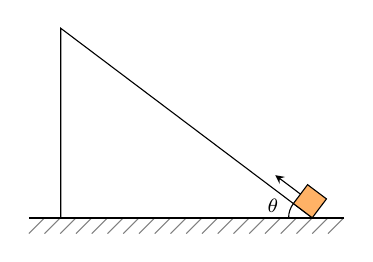
\begin{tikzpicture}[>=stealth,font=\scriptsize]
	\draw (0,0)--(143:4)--++(0,-2.4);
	\draw[fill=orange!60,rotate=-37] (0,0) rectangle(-.3,.3);
	\draw[->,rotate=-37] (-.3,.15)--(-.7,.15);
	\draw (-.3,0) arc(180:143:.3);
	\node at(-.5,.15){\(\theta\)};
	\foreach \x in {-3.6,-3.4,...,.4}
		\draw[gray] (\x,-.2)--++(.2,.2);
	\draw[thick] (-3.6,0)--(.4,0);
\end{tikzpicture}
\begin{answer}
    （1）\qty{4}{m}（2）\(\sqrt{2} + 1\) \qty{}{s}（3）\qty{4}{m/s}
\end{answer}